\documentclass[main.tex]{subfiles}

\begin{document}

  \section{Intersections}\label{sec:intersections}

  In \S \ref{m-subsec:cycles_homo} we presented a generating set $C$ for $\homo$.
  The formulas in Theorem \ref{m-thm:intsec_numb} explicitly determine the
  intersection matrix $K_C$ and
  the rest of the section is concerned with its proof.


  Since we generate $\homo$ with elementary cycles $\cyab$ and their shifts $\cyab^{(k)}$,
  we only need to know intersections between them. A further restriction is that by construction
  of the spanning tree we only need to
  consider intersections $\cyab\circ\cycd$ such that $c$ is either $a$ or $b$

  \begin{thm}[Intersection numbers]\label{thm:intsec_numb}
      Let $a,b,c,d\in X$ be branch points, and $\cyabl, \cycdk$ be in $C$.

      Then
      \begin{equation}
          \left(\cyab^{(k)} \circ \cycd^{(l)}\right)
          = \begin{cases}
              1  &\text{ if } l-k \equiv s_+ \bmod m\\
              -1 &\text{ if } l-k \equiv s_- \bmod m\\
              0 \text{ otherwise}
          \end{cases}
      \end{equation}
      where $s_+$, $s_-$ are given by the following table, which covers all
      cases occuring in the algorithm
      \begin{center}
      \begin{tabular}{lll}
          \toprule
          $(a,b),(c,d)$
          %$\cyab \circ \cycd$
          & $s_+$ & $s_-$ \\
          \midrule
          $a=c$ and $b=d$
          %$\cyab \circ \cyab$
          & $1$ & $-1$ \\
          $b=c$
          %$\cyab \circ \cybd$
          & $-s(b)$ & $1-s(b)$ \\
          $a=c$ and $\rho>0$
          %$\cyab \circ \cyad$ and $\rho>0$
          & $1-s(a)$ & $-s(a)$ \\
          $a=c$ and $\rho<0$
          %$\cyab \circ \cyad$ and $\rho<0$
          & $-s(a)$ & $-1-s(a)$\\
          $\set{a,b}\cap\set{c,d}=\varnothing$ & \multicolumn{2}{c}{no intersection} \\
          \bottomrule
      \end{tabular}
      \end{center}
      and where $s(x)\in\Z$ for $x\in\set{a,b}$ is given by
      \begin{equation}
          s(x) = \frac{(d-1)\rho+m(\arg \ytcd(x)-\arg\ytab(x))}{2π}
          +\delta_{a=c}\frac{1}2
      \end{equation}
     and
      \begin{equation}
          \rho = \arg(d-c) - \arg(b-a).
      \end{equation}
 \end{thm}

 \todo Notice $\ytab(a) = \prod_{x\neq a,b}(\frac{2x-2a}{b-a})^{\frac1m}$, and
 $s(x)$ can also be written
      \begin{equation}
      2π s(x) = (d-1)\rho
      + \sum_{x_k\neq c,d}\arg \frac{c-x_k}{d-c}
      - \sum_{x_k\neq a,b}\arg \frac{x-x_k}{b-a}
      \end{equation}

  \begin{proof}\let\qed\relax
   \begin{itemize}
    \item[($i$)] $P = (x,y) \in \cyabl \cap \cycdk   \Rightarrow  x \in [a,b] \cap [c,d]$.
   \end{itemize}
  \end{proof}

  In order to prove ($ii$) and ($iii$) we have to introduce some more machinery. Recall from \S \ref{m-subsec:roots_branches} that $\yab$ and $\ycd$ are analytic branches of $\cu$ on the open sets
  $\vab$ and $\vcd$ respectively. \abstandl
  We choose a common point $x \in V = \vab \cap \vcd$ and determine $s  = s(\cyab,\cycd,x) \in \Z/m\Z$  such that
  \begin{align}
   \frac{\ycd(x)}{\yab(x)} = \zeta^s .
  \end{align}
  We say $s  = s(\cyab,\cycd,x)$ is the \emph{shfiting number of $\cyab$ and $\cycd$ at $x$}.
  This definition naturally extends to shifts of elementary cycles via
\begin{align}\label{eq:shift_numb_rel}
  \frac{\zeta^k\ycd(x)}{\zeta^l\yab(x)} = \zeta^{s+k-l} \quad \imp \quad s(\cyabl,\cycdk,x) = s(\cyab,\cycd,x) + k - l.
\end{align}
 Hence, everything can be computed using only elementary cycles. \abstandl
 Within our setting, the shifting number $s=s(\cyab,\cycd,x)$  can be interpreted as '$\cyab$ running $s$ sheets above $\cycd$ at the point $x$'.
 Due to $\yab$ and $\yab$ being analytic, the shifting number is constant on connected open subsets of $V$. Moreover, the intersection number must be independent of the choice of that subset. \abstandl
 Thus,
 this information can be used to determine
 the intersection number graphically by continously deforming the cycles such that $(x,\yab(x)) \in \cyab$ and $(x,\ycd(x)) \in \cycd$.

   \begin{proof}(continued)
   \begin{itemize}
    \item[($ii$)] Here, we have that $[a,b] = [c,d]$. Hence, we can take $x = \frac{b+a}{2} \in  ]a,b[  \subset V = \vab$. We obtain the shifting number as
    \begin{align*}
      s(\cyabl,\cyab^{(k)},x) = s(\cyab,\cyab,x) + k - l = k - l.
    \end{align*}
    Obviously, we have that $\left(\cyabl \circ \cyab^{(k)}\right) = 0$ for $k - l \not\in \{ 0, \pm 1\}$. For the remaining cases, see Figure \ref{m-fig:int_self_shift} below.
    Illustrated are the cycles $\cyabl$ (black),
      $\cyab^{(l+1)}$ (red) and $\cyab^{(l-1)}$ (green).
    \begin{figure}[H]
      \begin{center}
   % Tikz File 'tikz_pic_3.tex'

%     \draw [densely dashed] (4.0,3) -- (5.2,3);  \draw [densely dashed] (8.8,3) -- (10,3); \draw (5.2,3) circle (1.3pt); \draw (8.8,3) circle (1.3pt);
%      
% \draw (4.5,3) .. controls (4.5,2.4) and (6,2.6) .. (7,3) [halfarrow2];
% \draw (7,3) .. controls (8,3.4) and (9.5,3.6) .. (9.5,3) [halfarrow2];
% 
%    \draw [densely dashed] (4,1) -- (5.2,1);  \draw [densely dashed] (8.8,1) -- (10,1); \draw (5.2,1) circle (1.3pt); \draw (8.8,1) circle (1.3pt);
% \draw (4.5,1) .. controls (4.5,1.6) and (6,1.4) .. (7,1) [halfarrow1];
% \draw (7,1) .. controls (8,0.6) and (9.5,0.4) .. (9.5,1) [halfarrow1];

\begin{tikzpicture}
% Sheet 4
     \draw [densely dashed] (-3,3) -- (-1.8,3); 
     \draw [densely dashed] (3,3) -- (1.8,3); 
     \draw (-1.8,3) circle (1.3pt); 
     \draw (1.8,3) circle (1.3pt);
    \draw[red] (-2.5,3) .. controls (-2.5,3.6) and (-1,3.4) .. (0,3) [halfarrow2];
     \draw[red] (0,3) .. controls (1,2.6) and (2.5,2.4) .. (2.5,3) [halfarrow2];

    %\draw (-1.8,2) node {$a$};  \draw (1.8,2) node {$b$};

     % Sheet 3
  \draw [densely dashed] (-3,1) -- (-1.8,1); 
     \draw [densely dashed] (3,1) -- (1.8,1); 
     \draw (-1.8,1) circle (1.3pt); 
     \draw (1.8,1) circle (1.3pt);
    \draw[red] (-2.5,1) .. controls (-2.5,1.6) and (-1,1.4) .. (0,1) [halfarrow1];
     \draw[red] (0,1) .. controls (1,0.6) and (2.5,0.4) .. (2.5,1) [halfarrow1];
    \draw (-2.5,1) .. controls (-2.5,0.6) and (-1,0.4) .. (0,1) [halfarrow2];
     \draw (0,1) .. controls (1,1.6) and (2.5,1.4) .. (2.5,1) [halfarrow2];

    % Intersection
    \draw (0,1) node[cross=3pt,black]{};
    \draw (0,1.3) node {$+1$};
     \draw (-1.8,0) node {$a$};  \draw (0,0) node {$\pr^{-1}(\xt)$}; \draw (1.8,0) node {$b$};

    % Sheet 2
\draw [densely dashed] (-3,-1) -- (-1.8,-1); 
     \draw [densely dashed] (3,-1) -- (1.8,-1); 
     \draw (-1.8,-1) circle (1.3pt); 
     \draw (1.8,-1) circle (1.3pt);
    \draw (-2.5,-1) .. controls (-2.5,-0.4) and (-1,-0.6) .. (0,-1) [halfarrow1];
     \draw (0,-1) .. controls (1,-1.4) and (2.5,-1.6) .. (2.5,-1) [halfarrow1];
    \draw [green] (-2.5,-1) .. controls (-2.5,-1.4) and (-1,-1.6) .. (0,-1) [halfarrow2];
     \draw [green] (0,-1) .. controls (1,-0.4) and (2.5,-0.6) .. (2.5,-1) [halfarrow2];

    % Intersection
    \draw (0,-1) node[cross=3pt,black]{};
    \draw (0,-1.3) node {$-1$};

     %\draw (-1.8,-2) node {$a$};  \draw (1.8,-2) node {$b$};

    % Sheet 1
  \draw [densely dashed] (-3,-3) -- (-1.8,-3); 
     \draw [densely dashed] (3,-3) -- (1.8,-3); 
     \draw (-1.8,-3) circle (1.3pt); 
     \draw (1.8,-3) circle (1.3pt);
    \draw[green] (-2.5,-3) .. controls (-2.5,-2.4) and (-1,-2.6) .. (0,-3) [halfarrow2];
     \draw[green] (0,-3) .. controls (1,-3.4) and (2.5,-3.6) .. (2.5,-3) [halfarrow2];
\end{tikzpicture}
      \end{center}
    \caption{Intersections of self-shifts.}
    \label{fig:int_self_shift}
\end{figure}
   \item[($iii$)]
  In the case $[a,b] \cap [c,d] = \{ x_0 \}$ we cannot compute the shifting number at $x_0$ directly, since $x_0 \not\in V = \vab \cap \vcd$. Instead, we choose a point $\xt$ on the bissectrix of
  $[a,b]$ and $[c,d]$, close enough to $x_0$, such that $[\xt,x_0[  \subset  V$. Then, for all $x \in [\xt,x_0[$ we compute the shifting number $s = s(\cyab,\cycd,x)$ as
  \begin{align}
   \zeta^s & = \frac{\ycd(x)}{\yab(x)} = \frac{(1- \ucd(x)^2)\mr (d-c)^{\frac{d}{m}}\ytcd(x) }{(1-\uab(x)^2)\mr (b-a)^{\frac{d}{m}}\ytab(x)} \\
   %\Rightarrow \frac{2\pi s}{m} = \arg \left( \frac{(1- u_{c,d}(x)^2)\mr}{(1-u_{a,b}(x)^2)\mr} \right) + \arg \left( \frac{(d-c)^{\frac{d}{m}} \ytcd(x)}{(b-a)^{\frac{d}{m}} \ytab(x)} \right) \\
   \Rightarrow  s & = \frac{1}{2\pi} \left( \arg \left( \frac{(1- \ucd(x)^2)}{(1-\uab(x)^2)} \right) + m \cdot \arg \left( \frac{(d-c)^{\frac{d}{m}} \ytcd(x)}{(b-a)^{\frac{d}{m}}
   \ytab(x)} \right) \right)
  \end{align}
  Letting $x$ tend to $x_0$ on the bissectrix and taking
  \todo{this must be done actually}
  \begin{align}
   \theta = \lim_{x \rightarrow x_0} \arg \left( \frac{(1- \ucd(x)^2)}{(1-\uab(x)^2)} \right)
  \end{align}
  we obtain equation \eqref{m-eq:shift_numb}. In any of the cases, this limit exists and it depends only on the choice of $\xt$. We will now proof ($iii$) for one of these cases.


  \begin{center}
   \underline{Case: $x_0 = b = c$}
  \end{center}
  As you can see in Figure \ref{m-fig:set_v} the set $V$ is not connected, but the disjoint union of two open sets that are seperated by the local branch cuts. Here, we choose $\xt$ on the upper bissectrix.
   \begin{figure}[H]
      \begin{center}
   % Tikz File 'tikz_pic_4.tex'
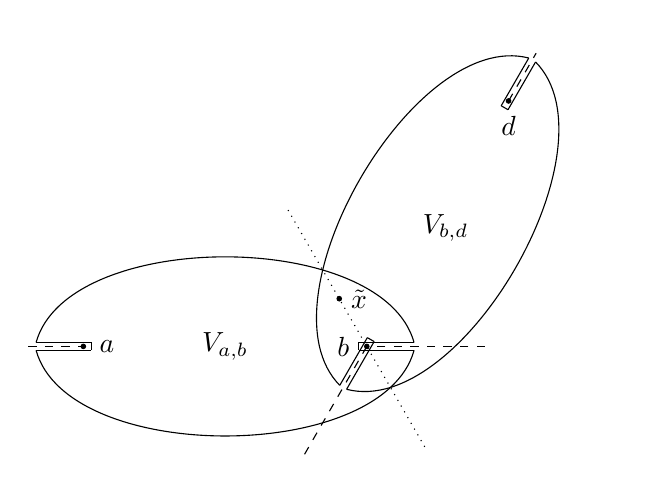
\begin{tikzpicture}

    

% \draw (-1.8,1.0) node {$\Phi(\tilde{\alpha})$};  \draw (2,-1.3) node {$\Phi(\tilde{\beta})$};
  \draw (-3.3,0) node {$a$};  \draw (-0.3,0) node {$b$}; \draw (-1.8,0) node {$V_{a,b}$};
  \filldraw [black] (-3.6,0) circle (0.8pt); \filldraw [black] (0,0) circle (0.8pt);
    \draw [dashed] (-4.3,0) -- (-3.6,0);   \draw [dashed] (1.5,0) -- (0,0);
    \draw (-4.2,0.05) .. controls (-3.8,1.5) and (0.2,1.5) .. (0.6,0.05);
    \draw (-4.2,-0.05) .. controls (-3.8,-1.5) and (0.2,-1.5) .. (0.6,-0.05);
    \draw (-4.2,-0.05) -- (-3.5,-0.05); \draw (0.6,-0.05) -- (-0.1,-0.05);
    \draw (-4.2,0.05) -- (-3.5,0.05); \draw (0.6,0.05) -- (-0.1,0.05);
    \draw (-3.5,0.05) -- (-3.5,-0.05); \draw (-0.1,0.05) -- (-0.1,-0.05);
    
  \filldraw [black] (1.8,3.117) circle (0.8pt); 
  \draw (1.8,2.8) node {$d$}; \draw (1.0,1.5) node {$V_{b,d}$};
  \draw [dashed] (1.8,3.117) -- (2.15,3.723); \draw [dashed] (0,0) -- (-0.8,-1.386);
  \draw [rotate=240,shift={(0,0)}] (-4.2,0.05) .. controls (-3.8,1.5) and (0.2,1.5) .. (0.6,0.05);
  \draw [rotate=240,shift={(0,0)}] (-4.2,-0.05) .. controls (-3.8,-1.5) and (0.2,-1.5) .. (0.6,-0.05);
  \draw [rotate=240,shift={(0,0)}] (-4.2,-0.05) -- (-3.5,-0.05);  \draw [rotate=240,shift={(0,0)}] (0.6,-0.05) -- (-0.1,-0.05);
    \draw [rotate=240,shift={(0,0)}](-4.2,0.05) -- (-3.5,0.05); \draw [rotate=240,shift={(0,0)}] (0.6,0.05) -- (-0.1,0.05);
       \draw [rotate=240,shift={(0,0)}] (-3.5,0.05) -- (-3.5,-0.05); \draw [rotate=240,shift={(0,0)}] (-0.1,0.05) -- (-0.1,-0.05);
       
  \draw [dotted] (-1,1.732) -- (0.75,-1.3);
  \filldraw [black] (-0.35,0.606) circle (0.8pt); \draw (-0.1,0.6) node {$\tilde{x}$};


 
\end{tikzpicture}

      \end{center}x
    \caption{The set $V = \vab \cap \vbd$.}
    \label{fig:set_v}
\end{figure}
  With $\rho = \arg\left(\frac{b-a}{d-b}\right)$ we have that
  \begin{align*}
   & \arg (1+\ubd(x)) = \frac{\pi+\rho}{2} \quad \text{for all}  x \in [\xt,x_0[,\\
   & \arg (1-\uab(x)) = -\frac{\pi+\rho}{2} \quad \text{for all}  x \in [\xt,x_0[,\\
   & \arg (1-\ubd(x_0)) = 0,\\
   & \arg (1+\uab(x_0))= 0,
  \end{align*}
  and therefore
  \begin{align*}
   \theta = \frac{\pi+\rho}{2} - \left(-\frac{\pi+\rho}{2}\right) = \pi + \rho.
  \end{align*}
  Assuming that the shifting number $s=s(\cyab,\cycd,\xt)$ is computed as above, we can now determine the intersections graphically. \abstandl
  As before, the only interesting cases
  are $s \in \{0,\pm 1\}$. Figure \ref{m-fig:int_b=c} displays the cycles $\cyab$ (black) and $\cycd$ in green ($s=1$), gray ($s=0$) and red ($s=-1$).
  We can read off the intersection numbers
  \begin{align*}
    \left(\cyab \circ \cycd\right) = \begin{cases}
                                          +1, \quad & \text{if} \quad s=0,\\
                                          -1, \quad & \text{if} \quad s=1,\\
                                          \quad\!0, \quad & \text{otherwise}.
                                         \end{cases}
  \end{align*}
  The relation \eqref{m-eq:shift_numb_rel} extends this to $\left(\cyabl \circ \cycdk\right)$ as claimed.
  \begin{figure}[H]
      \begin{center}
   \begin{tikzpicture}

  \draw (-3.6,2) node {$a$};  \draw (0,2) node {$b$};  \draw (1.8,5.117) node {$d$}; 
  
  
% Intersections
    \draw (-0.75,4.25) node[cross=3pt,black,rotate=80]{};
    \draw (-1,4.5) node {$-1$};    
      \draw (-0.35,0.606) node[cross=3pt,black,rotate=60]{};
    \draw (0.0,0.5) node {$+1$}; 

% Sheet 3
  \filldraw [black] (-3.6,8) circle (0.8pt); 
  \filldraw [black] (0,8) circle (0.8pt);   
  \filldraw [black] (1.8,11.117) circle (0.8pt); 
  \draw [dashed] (-4.3,8) -- (-3.6,8); 
  \draw [dashed] (1.8,11.117) -- (2.15,11.723);
  \draw [dashed] (0,8) -- (0.5,7.134); 
  \draw [green] (1.95,11.377) .. controls (0.5,12) and (1.5,8.5) .. (0.35,7.4) [halfarrow1];

  
  
% Sheet 2
  \filldraw [black] (-3.6,4) circle (0.8pt); 
  \filldraw [black] (0,4) circle (0.8pt);   
  \filldraw [black] (1.8,7.117) circle (0.8pt); 
  \draw [dashed] (-4.3,4) -- (-3.6,4); 
  \draw [dashed] (1.8,7.117) -- (2.15,7.723);
  \draw [dashed] (0,4) -- (0.5,3.134); 
  \draw (-3.9,4) .. controls (-2.5,3) and (0.8,5.5) .. (0.18,3.7) [halfarrow2];
  \draw [green] (1.95,7.377) .. controls (2,6.5) and (2,5.5) .. (-0.35,4.606) [halfarrow2];
  \draw [green] (-0.35,4.606) arc(110:310:0.7cm) [halfarrow2];
  \draw [gray] (1.95,7.377) .. controls (0.5,8) and (1.5,4.5) .. (0.35,3.4) [halfarrow1];
 
 
% Sheet 1
\filldraw [black] (-3.6,0) circle (0.8pt); 
\filldraw [black] (0,0) circle (0.8pt);   
\filldraw [black] (1.8,3.117) circle (0.8pt); 
% \filldraw [black] (-0.35,0.606) circle (0.8pt);
    \draw [dashed] (-4.3,0) -- (-3.6,0);  
    \draw [dashed] (1.8,3.117) -- (2.15,3.723); 
    \draw [dashed] (0,0) -- (0.5,-0.866);
    \draw (-3.9,0) .. controls (-3,0.5) and (0.2,1.5) .. (-0.35,0.606) [halfarrow1];
    \draw [gray] (1.95,3.377) .. controls (2.8,3) and (2,1.5) .. (-0.35,0.606) [halfarrow2];
    \draw (-0.35,0.606) arc(150:270:0.6cm) [halfarrow1];
        \draw [gray] (-0.35,0.606) arc(110:310:0.7cm) [halfarrow2];
      \draw [blue] (1.95,3.377) .. controls (0.5,4) and (1.5,0.5) .. (0.35,-0.6) [halfarrow1];


% Sheet 0
\filldraw [black] (-3.6,-4) circle (0.8pt); 
\filldraw [black] (0,-4) circle (0.8pt);   
\filldraw [black] (1.8,-0.883) circle (0.8pt); 
    \draw [dashed] (-4.3,-4) -- (-3.6,-4);  
    \draw [dashed] (1.8,-0.883) -- (2.15,-0.277); 
    \draw [dashed] (0,-4) -- (0.5,-4.866);
    \draw [blue] (-0.35,-3.394) arc(110:310:0.7cm) [halfarrow2];
    \draw [blue] (1.95,-0.623) .. controls (2,-1.5) and (2,-2.5) .. (-0.35,-3.394) [halfarrow2];
 
\end{tikzpicture}
      \end{center}
    \caption{Intersections for $b=c$ and $s \in \{1,0,-1\}$.}
    \label{fig:int_b=c}
\end{figure}
 \end{itemize}
 \todo Other cases?
  \end{proof}



%  \begin{defn}\label{def:shift_numb}
%  Let $\cyab, \cycd \in C$ be elementary cycles and let $V = V_{a,b} \cap V_{c,d}$. Then, $\yab$ and $\ycd$ are analytic functions with no zeros on $V$. For each $x \in V$ there
%  exists an $s \in \Z/m\Z$ such that
%  \begin{align}
%    \frac{\ycd(x)}{\yab(x)} = \zeta^s .
%  \end{align}
%  We say $s  = s(\cyab,\cycd,x)$ is the \emph{shfiting number of $\cyab$ and $\cycd$ at $x$}.
%  \end{defn}
%  This definition naturally extends to shifts of elementary cycles via
%  \begin{align}
%    \frac{\zeta^k\ycd(x)}{\zeta^l\yab(x)} = \zeta^{s+k-l} \quad \imp \quad s(\cyabl,\cycdk,x) = s(\cyab,\cycd,x) + k - l.
%  \end{align}


%  Note that the set $V$ is not connected. It is split up into two disjoint open subsets by the local branch cuts. Although the shifting number is not constant on $V$, it is constant on its
%  connected components.
%
%  However, computing the shifting number for \emph{one} point $x \in V$ is sufficient to determine all the intersections $\left(  \cyabl \circ \cycdk \right)$.
%
%      We can compute the shiftung number for all elementary cycles $\cyab, \cycd \in C$:
%
%     \begin{thm}\label{thm:shift_numb}
%     Assume $[a,b] \cap [c,d] = \{x\}$. With notations as above and $\tau = \arg \left( \frac{d-c}{b-a} \right)$ we have that
%      \begin{align}\label{eq:shift_numb}
%        s(\alpha,\beta) = \frac{1}{2\pi} \left( \theta +  m \cdot \arg \left( \frac{(b-a)^{\frac{d}{m}} \ytab(x)}{(d-c)^{\frac{d}{m}} \ytcd(x)} \right) \right) \in \Z/m\Z,
%      \end{align}
%      where
%       \begin{align*}\theta = \begin{cases}
%                                -\pi+\tau, \quad \text{if} \quad \tau < 0 \quad \text{and} \quad (x = b = c \quad \text{or} \quad x = a = d),\\
%                               \quad\! \pi-\tau, \quad \text{if} \quad \tau \ge 0 \quad \text{and} \quad (x = b = c \quad \text{or} \quad x = a = d),\\
%                               \hspace{0.7cm} -\tau, \quad \text{if} \quad x = a = c \quad \text{or} \quad x = b = d,\\
%                               \hspace{1cm} 0, \quad \text{if} \quad x  \in  ]a,b[ \cap ]c,d[.
%                              \end{cases}
%      \end{align*}
%     \end{thm}
%     \begin{proof}
%      See \S \todo ref.
%     \end{proof}
%
%      Using this information, we obtain the intersection numbers graphically by using visualizations of $\alpha$ on $\beta$ running on different sheets.
%      However, if we find homologous cycles, whose projections do not intersect, their lifts to the surface cannot intersect.

%     At a common point $p$, that is no branch points, the notion of sheets makes sense and there exists an $s \in \Z/N\Z$ such that. This means that above the point $p$
%      $\beta_0$ runs $s$ sheets above $\alpha_0$. We will call $s = s(\alpha,\beta)$ the \textit{shifting number} of $\alpha$ and $\beta$ at $p$.
%     If $p$ is a branch point, we choose homologous paths whose $x$-projections intersect at a non-branch point and take a limit.



%        \begin{split}
%         (\cyabl \circ \cycdk) =
%         \begin{cases}
%             \hspace*{0.95cm} -1, \quad & \text{if} \quad s=0 \quad \text{and} \quad (x = b = c \quad \text{or} \quad x = a = d),\\
%       \hspace*{0.95cm} +1, \quad &\text{if} \quad s=-1 \quad \text{and} \quad (x = b = c \quad \text{or} \quad x = a = d),\\
%           \quad\! \sgn(\tau), \quad & \text{if} \quad s=0 \quad \text{and} \quad (x = a = c \quad \text{or} \quad x = b = d),\\
%             -\sgn(\tau), \quad & \text{if} \quad s=-\sgn(\tau) \quad \text{and} \quad (x = a = c \quad \text{or} \quad x = b = d),\\
%           \hspace*{0.95cm} +1, \quad &\text{if} \quad s=1 \quad \text{and} \quad [a,b] = [c,d],\\
%           \hspace*{0.95cm} -1, \quad &\text{if} \quad s=-1 \quad \text{and} \quad [a,b] = [c,d],\\
%          \hspace*{0.95cm}  \quad\! 0, \quad &\text{otherwise}.
%         \end{cases}
%        \end{split}
%       \end{align}

\end{document}
